\documentclass[border=5pt]{standalone}
\usepackage{fontspec,unicode-math}
\setmainfont{Noto Serif}
\setmathfont{STIXTwoMath-Regular.otf}
\usepackage{tikz}
\usetikzlibrary{arrows.meta,calc,patterns,decorations.markings}
\definecolor{Ink}{HTML}{000000}
\tikzset{ax/.style={draw=Ink,line width=.65pt,-{Latex[length=2.2mm,width=1.25mm]}},
lev/.style={draw=Ink,line width=1.25pt,line cap=butt},
fine/.style={draw=Ink,line width=.60pt},
band/.style={draw=Ink,line width=.62pt},
sol/.style={draw=Ink,line width=1.35pt,line cap=round,line join=round},
ray/.style={draw=Ink,line width=.72pt,-{Latex[length=2.0mm,width=1.15mm]}},
dim/.style={draw=Ink,line width=.60pt,{Latex[length=1.7mm,width=.95mm]}-{Latex[length=1.7mm,width=.95mm]}},
lab/.style={text=Ink,font=\fontsize{13}{16}\selectfont,inner sep=1.1pt},
small/.style={text=Ink,font=\fontsize{11}{13}\selectfont,inner sep=1.0pt}}
\pagestyle{empty}
\def\datadir{data}
\IfFileExists{data/F20_1_heat.dat}{}{\def\datadir{../data}}
\begin{document}
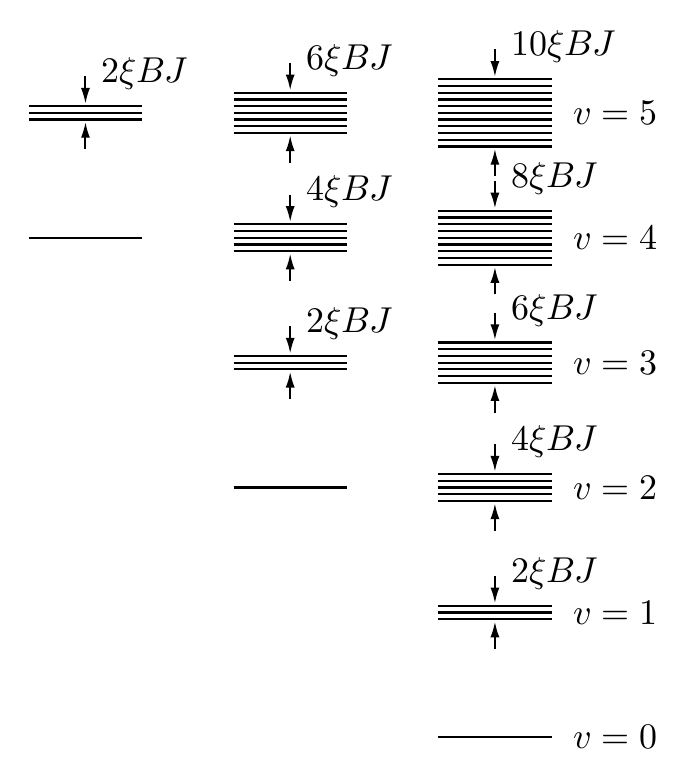
\begin{tikzpicture}[x=1cm,y=1.22cm]
% R2 CP04: vertical magnification 1.22 preserves all relative level locations and clears dimension labels.
% Each row: L=v,v-2,... ; each multiplet M=-L,...,+L; shift = M*xi*B*J.
\draw[band,line width=.80pt] (5.63,0.45000)--(7.069999999999999,0.45000);
\node[lab,anchor=west] at (7.30000,0.45000) {$v=0$};
\draw[band,line width=.80pt] (5.63,1.68000)--(7.069999999999999,1.68000);
\draw[band,line width=.80pt] (5.63,1.75000)--(7.069999999999999,1.75000);
\draw[band,line width=.80pt] (5.63,1.82000)--(7.069999999999999,1.82000);
\draw[ray] (6.35,2.13000)--(6.35,1.84500);
\draw[ray] (6.35,1.37000)--(6.35,1.65500);
\node[lab,anchor=south west] at (6.51000,1.95000) {$2\xi BJ$};
\node[lab,anchor=west] at (7.30000,1.75000) {$v=1$};
\draw[band,line width=.80pt] (5.63,2.91000)--(7.069999999999999,2.91000);
\draw[band,line width=.80pt] (5.63,2.98000)--(7.069999999999999,2.98000);
\draw[band,line width=.80pt] (5.63,3.05000)--(7.069999999999999,3.05000);
\draw[band,line width=.80pt] (5.63,3.12000)--(7.069999999999999,3.12000);
\draw[band,line width=.80pt] (5.63,3.19000)--(7.069999999999999,3.19000);
\draw[ray] (6.35,3.50000)--(6.35,3.21500);
\draw[ray] (6.35,2.60000)--(6.35,2.88500);
\node[lab,anchor=south west] at (6.51000,3.32000) {$4\xi BJ$};
\draw[band,line width=.80pt] (3.0299999999999994,3.05000)--(4.47,3.05000);
\node[lab,anchor=west] at (7.30000,3.05000) {$v=2$};
\draw[band,line width=.80pt] (5.63,4.14000)--(7.069999999999999,4.14000);
\draw[band,line width=.80pt] (5.63,4.21000)--(7.069999999999999,4.21000);
\draw[band,line width=.80pt] (5.63,4.28000)--(7.069999999999999,4.28000);
\draw[band,line width=.80pt] (5.63,4.35000)--(7.069999999999999,4.35000);
\draw[band,line width=.80pt] (5.63,4.42000)--(7.069999999999999,4.42000);
\draw[band,line width=.80pt] (5.63,4.49000)--(7.069999999999999,4.49000);
\draw[band,line width=.80pt] (5.63,4.56000)--(7.069999999999999,4.56000);
\draw[ray] (6.35,4.87000)--(6.35,4.58500);
\draw[ray] (6.35,3.83000)--(6.35,4.11500);
\node[lab,anchor=south west] at (6.51000,4.69000) {$6\xi BJ$};
\draw[band,line width=.80pt] (3.0299999999999994,4.28000)--(4.47,4.28000);
\draw[band,line width=.80pt] (3.0299999999999994,4.35000)--(4.47,4.35000);
\draw[band,line width=.80pt] (3.0299999999999994,4.42000)--(4.47,4.42000);
\draw[ray] (3.7499999999999996,4.73000)--(3.7499999999999996,4.44500);
\draw[ray] (3.7499999999999996,3.97000)--(3.7499999999999996,4.25500);
\node[lab,anchor=south west] at (3.91000,4.55000) {$2\xi BJ$};
\node[lab,anchor=west] at (7.30000,4.35000) {$v=3$};
\draw[band,line width=.80pt] (5.63,5.37000)--(7.069999999999999,5.37000);
\draw[band,line width=.80pt] (5.63,5.44000)--(7.069999999999999,5.44000);
\draw[band,line width=.80pt] (5.63,5.51000)--(7.069999999999999,5.51000);
\draw[band,line width=.80pt] (5.63,5.58000)--(7.069999999999999,5.58000);
\draw[band,line width=.80pt] (5.63,5.65000)--(7.069999999999999,5.65000);
\draw[band,line width=.80pt] (5.63,5.72000)--(7.069999999999999,5.72000);
\draw[band,line width=.80pt] (5.63,5.79000)--(7.069999999999999,5.79000);
\draw[band,line width=.80pt] (5.63,5.86000)--(7.069999999999999,5.86000);
\draw[band,line width=.80pt] (5.63,5.93000)--(7.069999999999999,5.93000);
\draw[ray] (6.35,6.24000)--(6.35,5.95500);
\draw[ray] (6.35,5.06000)--(6.35,5.34500);
\node[lab,anchor=south west] at (6.51000,6.06000) {$8\xi BJ$};
\draw[band,line width=.80pt] (3.0299999999999994,5.51000)--(4.47,5.51000);
\draw[band,line width=.80pt] (3.0299999999999994,5.58000)--(4.47,5.58000);
\draw[band,line width=.80pt] (3.0299999999999994,5.65000)--(4.47,5.65000);
\draw[band,line width=.80pt] (3.0299999999999994,5.72000)--(4.47,5.72000);
\draw[band,line width=.80pt] (3.0299999999999994,5.79000)--(4.47,5.79000);
\draw[ray] (3.7499999999999996,6.10000)--(3.7499999999999996,5.81500);
\draw[ray] (3.7499999999999996,5.20000)--(3.7499999999999996,5.48500);
\node[lab,anchor=south west] at (3.91000,5.92000) {$4\xi BJ$};
\draw[band,line width=.80pt] (0.4299999999999995,5.65000)--(1.8699999999999994,5.65000);
\node[lab,anchor=west] at (7.30000,5.65000) {$v=4$};
\draw[band,line width=.80pt] (5.63,6.60000)--(7.069999999999999,6.60000);
\draw[band,line width=.80pt] (5.63,6.67000)--(7.069999999999999,6.67000);
\draw[band,line width=.80pt] (5.63,6.74000)--(7.069999999999999,6.74000);
\draw[band,line width=.80pt] (5.63,6.81000)--(7.069999999999999,6.81000);
\draw[band,line width=.80pt] (5.63,6.88000)--(7.069999999999999,6.88000);
\draw[band,line width=.80pt] (5.63,6.95000)--(7.069999999999999,6.95000);
\draw[band,line width=.80pt] (5.63,7.02000)--(7.069999999999999,7.02000);
\draw[band,line width=.80pt] (5.63,7.09000)--(7.069999999999999,7.09000);
\draw[band,line width=.80pt] (5.63,7.16000)--(7.069999999999999,7.16000);
\draw[band,line width=.80pt] (5.63,7.23000)--(7.069999999999999,7.23000);
\draw[band,line width=.80pt] (5.63,7.30000)--(7.069999999999999,7.30000);
\draw[ray] (6.35,7.61000)--(6.35,7.32500);
\draw[ray] (6.35,6.29000)--(6.35,6.57500);
\node[lab,anchor=south west] at (6.51000,7.43000) {$10\xi BJ$};
\draw[band,line width=.80pt] (3.0299999999999994,6.74000)--(4.47,6.74000);
\draw[band,line width=.80pt] (3.0299999999999994,6.81000)--(4.47,6.81000);
\draw[band,line width=.80pt] (3.0299999999999994,6.88000)--(4.47,6.88000);
\draw[band,line width=.80pt] (3.0299999999999994,6.95000)--(4.47,6.95000);
\draw[band,line width=.80pt] (3.0299999999999994,7.02000)--(4.47,7.02000);
\draw[band,line width=.80pt] (3.0299999999999994,7.09000)--(4.47,7.09000);
\draw[band,line width=.80pt] (3.0299999999999994,7.16000)--(4.47,7.16000);
\draw[ray] (3.7499999999999996,7.47000)--(3.7499999999999996,7.18500);
\draw[ray] (3.7499999999999996,6.43000)--(3.7499999999999996,6.71500);
\node[lab,anchor=south west] at (3.91000,7.29000) {$6\xi BJ$};
\draw[band,line width=.80pt] (0.4299999999999995,6.88000)--(1.8699999999999994,6.88000);
\draw[band,line width=.80pt] (0.4299999999999995,6.95000)--(1.8699999999999994,6.95000);
\draw[band,line width=.80pt] (0.4299999999999995,7.02000)--(1.8699999999999994,7.02000);
\draw[ray] (1.1499999999999995,7.33000)--(1.1499999999999995,7.04500);
\draw[ray] (1.1499999999999995,6.57000)--(1.1499999999999995,6.85500);
\node[lab,anchor=south west] at (1.31000,7.15000) {$2\xi BJ$};
\node[lab,anchor=west] at (7.30000,6.95000) {$v=5$};
\end{tikzpicture}
\end{document}
